% RoadWatch BD conference paper: DRAFT 1 (2026-11-05)
% Red text = a number that is not measured yet (Kaggle leaky/clean runs) or a decision for the authors.
% Compile on Overleaf (pdfLaTeX, IEEEtran is built in). Figures: paper/make_figures.py.
\documentclass[conference]{IEEEtran}
\IEEEoverridecommandlockouts
\usepackage[T1]{fontenc}
\usepackage{cite}
\usepackage{amsmath,amssymb}
\usepackage{graphicx}
\usepackage{booktabs}
\usepackage{multirow}
\usepackage{xcolor}
\usepackage{url}
\graphicspath{{figs/}}

\newcommand{\TBD}[1]{\textcolor{red}{#1}}   % pending result or author decision
\newcommand{\vid}[1]{\texttt{#1}}            % a BadODD video name

\begin{document}

\title{Same Video, Different Frame: Measuring Train--Test Leakage in a Bangladeshi Road Object Detection Benchmark}

\author{\IEEEauthorblockN{\TBD{[Author names --- to be added by the authors]}}
\IEEEauthorblockA{\TBD{[Department, University, City, Country]}\\
\TBD{[email]}}}

\maketitle

\begin{abstract}
Object detectors for Bangladeshi roads are increasingly trained and compared on BadODD, a dataset of frames
sampled from smartphone videos recorded from moving cars in nine districts. Its official
train/validation/test split is drawn by image, so frames of one video land in all three splits. We audit
this split and find that each of the 2,033 official test images has a training or validation frame from the
same video, a median of 59 source frames (one sampling step) away. To measure what this leakage does to
reported accuracy, we build a video-held-out re-split matched to the official split in size and class mix,
and a paired protocol in which two equally sized training sets, one containing other frames of the test
videos and one not, are evaluated on the same 1,019 test images. A COCO-pretrained RT-DETR cannot output
35\% of BadODD's test objects and reaches an mAP@50 of 0.245; fine-tuning on the official split raises this
to 0.663. Under the paired protocol, fine-tuned RT-DETR scores \TBD{X.XXX} with leaked frames and
\TBD{Y.YYY} without (difference \TBD{+D.DDD}, 95\% CI \TBD{[a, b]}, paired video-level bootstrap), and
YOLO11s \TBD{\ldots}. We release the split manifests and evaluation code, and recommend video-held-out
splits with video-level confidence intervals for any dataset built from video.
\end{abstract}

\begin{IEEEkeywords}
object detection, data leakage, evaluation protocol, autonomous driving, Bangladesh, dataset split
\end{IEEEkeywords}

% =====================================================================
\section{Introduction}

Road scenes in Bangladesh are dominated by vehicles that general-purpose detection datasets do not
contain: pedal rickshaws, CNG auto-rickshaws, battery rickshaws and locally built carriers share the road
with buses, trucks and dense pedestrian traffic. A detector pretrained on COCO~\cite{coco} has no class for
most of them. On the BadODD test split, 35\% of the annotated objects belong to classes that a COCO model
cannot output, and the CNG auto-rickshaws it does see are mostly reported as trucks or cars
(Section~\ref{sec:zeroshot}). Local datasets such as BadODD~\cite{badodd}, BNVD~\cite{bnvd} and
RSUD20K~\cite{rsud20k} were built to close this gap, and detectors fine-tuned on them report mAP values
between 0.6 and 0.85 on the datasets' own test splits~\cite{badodd,bnvd,rsud20k}.

How far such numbers transfer to new roads depends on how the test set was drawn. BadODD was collected by
recording videos from the front of moving cars and sampling one frame every one or two
seconds~\cite{badodd}. Its official split assigns these frames to training, validation and test at a
60:20:20 ratio by image. Consecutive sampled frames of one video show the same road, buildings, lighting and
often the same vehicles, so a random image split places near-copies of most test images in the training
set. This is a well-known failure of evaluation for grouped data~\cite{kaufman,kapoor,roberts}, and
near-duplicates have been shown to inflate scores in image classification~\cite{barz} and licence-plate
recognition~\cite{laroca}. For road object detection in Bangladesh it has, to our knowledge, not been
measured.

This paper measures it. Our contributions are:
\begin{itemize}
\item An audit of BadODD's official split (Section~\ref{sec:audit}): all 44 videos (identified from the
file names) appear in both training and validation, 42 of them also in test, and every test image has a
same-video training or validation frame a median of one sampling step away.
\item Two leakage-free protocols (Section~\ref{sec:protocols}): a video-held-out re-split whose size and
per-class box shares are matched to the official split, and a paired leaky/clean protocol that holds the test images,
training-set size, validation set and recipe fixed and changes only whether the training set contains other
frames of the test videos.
\item Measurements with a COCO-pretrained baseline and two fine-tuned detectors (RT-DETR-R18~\cite{rtdetr}
and YOLO11s~\cite{yolo11}), with confidence intervals that resample whole videos and a paired interval for
the leakage effect itself.
\item The split manifests and evaluation code, released at
\TBD{\url{https://github.com/muttakin210/roadwatch-bd}} \TBD{[authors: confirm the repository is public]}.
\end{itemize}

% =====================================================================
\section{Related Work}

\subsection{Road object detection in Bangladesh}
BadODD~\cite{badodd} provides 13 characteristic-based classes (for example \emph{three-wheeler} for pedal
rickshaws and \emph{auto rickshaw} for motorised three-wheelers) over frames from nine districts, day and
night; its authors report mAP values of 0.6 and 0.7 for YOLOv5 and YOLOv8 on their split. BNVD~\cite{bnvd}
collects 17,326 images of 17 native vehicle classes from 17 districts, splits them at random (70\% for
training) and reports an mAP@50 of 0.848 for YOLOv8. RSUD20K~\cite{rsud20k} provides 20,334
dashboard-camera images from more than 80 video sequences with 13 classes, and is the exception: it assigns
whole sequences to training, validation and test to avoid leakage, but does not measure what this changes.
Earlier collections such as DhakaAI~\cite{dhakaai} and Poribohon-BD~\cite{poribohon} focus on Dhaka traffic
and on vehicle classification. On the model side, YOLO variants have been compared on Bangladeshi traffic
images~\cite{alamgir,yoloeval}, and RT-DETR fine-tuned on BadODD reached mAP@50 of 0.415 and 0.282 on the
public and private parts of a competition test set~\cite{rtdetrbd}. Apart from RSUD20K, these works report
results on random image splits or on test sets whose relation to the training videos is not described, and
none measures how much of a score comes from shared videos.

\subsection{Leakage and grouped evaluation}
Kaufman et al.~\cite{kaufman} formalise leakage as information in the training data that would not be
available when the model is used, and Kapoor and Narayanan~\cite{kapoor} find it behind many irreproducible
results, including non-independence between training and test samples. In vision, Barz and
Denzler~\cite{barz} found near-duplicates of 3.3\% and 10\% of the CIFAR-10 and CIFAR-100 test images in the
training sets, and Laroca et al.~\cite{laroca} showed that removing images of the same licence plate from
both sides of a split lowers recognition rates and can reorder models. Recht et al.~\cite{recht} observed
accuracy drops on freshly collected test sets even without exact overlap. For data with group structure,
Roberts et al.~\cite{roberts} recommend blocking the split by the grouping variable. Several driving
datasets avoid the problem by design: Cityscapes~\cite{cityscapes} separates its splits by city, and
BDD100K~\cite{bdd100k} annotates one key frame per video. For the uncertainty of scores computed on grouped
test sets, resampling whole clusters~\cite{fieldwelsh} rather than individual samples~\cite{efron} keeps
the confidence interval honest.

% =====================================================================
\section{Dataset and Leakage Audit}
\label{sec:audit}

\subsection{BadODD and the label set}
We use the BadODD release on Zenodo (record 13823687, CC BY 4.0). It contains 10,032 labelled images; the
dataset paper describes 9,825~\cite{badodd}. File names have the form \vid{<video>\_<frame>}, for example
\vid{dhaka2\_10320}, where the frame number counts frames of the source video. Grouping by the prefix gives
44 videos from nine locations, five of them recorded at night (1,705 images). We treat each prefix as one
video; if a prefix covered several recordings, grouping by it would only make our splits more conservative.

The project this work belongs to uses a 15-class label set for Bangladeshi traffic; Table~\ref{tab:classes}
shows how BadODD's classes map onto the ten that occur in it. BadODD defines its classes by
characteristics; \emph{auto rickshaw} is any motorised three-wheeler, gas or electric~\cite{badodd}, so CNG
auto-rickshaws and battery rickshaws share one class. The \emph{train} and
\emph{wheelchair} classes (one and three boxes in the paper's statistics~\cite{badodd}) are dropped.

\begin{table}[t]
\centering
\caption{BadODD classes mapped to our label set, with box counts over all 10,032 images.}
\label{tab:classes}
\begin{tabular}{@{}llr@{}}
\toprule
Our class & BadODD class(es) & Boxes \\
\midrule
person & person & 31,016 \\
cng\_autorickshaw & auto rickshaw & 17,820 \\
rickshaw & three-wheeler & 9,664 \\
car & car & 6,336 \\
motorcycle & motorbike & 6,272 \\
truck & truck & 3,863 \\
bus & bus & 3,096 \\
bicycle & bicycle & 1,195 \\
ambulance & priority vehicle & 369 \\
other & cart vehicle, construction vehicle & 279 \\
\midrule
--- & train, wheelchair (dropped) & --- \\
\bottomrule
\end{tabular}
\end{table}

\subsection{How the official split leaks}
The official split has 5,967 training, 2,032 validation and 2,033 test images. All 44 videos have frames in
training and validation, and 42 in test. For every test image we find the nearest training or validation
frame of the same video, measured in source-video frames. Every one of the 2,033 test images has such a
frame. The median distance is 59 frames, which is also the median spacing between consecutive labelled
frames of a video: the nearest training frame of a typical test image is the next or previous sampled frame.
28\% of the test images are within 30 frames and 85\% within 60 (Fig.~\ref{fig:leak}b). Fig.~\ref{fig:leak}a
shows the first 40 labelled frames of one video: the official split interleaves training, validation and
test frames along the drive.

\begin{figure}[t]
\centering
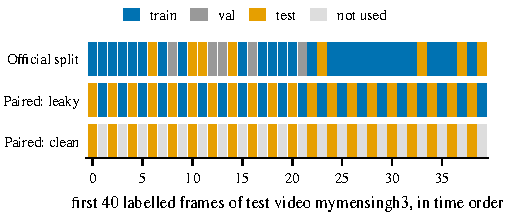
\includegraphics[width=\columnwidth]{split_timeline}\\[2pt]
\small (a)\\[4pt]
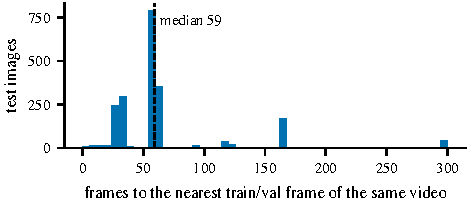
\includegraphics[width=\columnwidth]{leak_gaps}\\[2pt]
\small (b)
\caption{(a) The first 40 labelled frames of test video \vid{mymensingh3} and the split each protocol puts
them in. The official split interleaves training and test frames; the paired protocol uses every other
frame for testing and either trains on the frames in between (leaky) or not at all (clean). (b) For each of
the 2,033 official test images, the distance in source-video frames to the nearest training or validation
frame of the same video.}
\label{fig:leak}
\end{figure}

% =====================================================================
\section{Leakage-Free Protocols}
\label{sec:protocols}

\subsection{Video-held-out split}
We pool the official splits and assign whole videos to training, validation and test. Out of 20,000 random
greedy assignments (each video goes to the split with the largest relative deficit of images) followed by
hill-climbing over single-video moves and swaps, we keep the one that minimises
\begin{equation}
\sum_{s} \Big[ \tfrac{|n_s - t_s|}{t_s}
  + \tfrac{1}{K}\sum_{k} \tfrac{|b_{s,k} - t_s|}{t_s}
  + \max_{k} \tfrac{|b_{s,k} - t_s|}{t_s}
  + 0.1\,\tfrac{|m_s - t_s|}{t_s} \Big] + 10\,P,
\end{equation}
where for split $s$, $t_s$ is its share of images in the official split, $n_s$ its share of images,
$b_{s,k}$ its share of the boxes of class $k$, $m_s$ its share of night images, and $P$ counts the classes
missing from a split plus the splits without night footage. Night footage is weighted low because it comes
in five videos, two of them with 695 and 869 labelled images, so its share can only be matched roughly. The result
(Table~\ref{tab:splits}) has 21, 11 and 12 videos and 5,967, 2,031 and 2,034 images; each class receives
between 14\% and 28\% of its boxes in the test split. The assignment is stored as a manifest, so the split
is rebuilt identically on any machine.

\subsection{Paired leaky/clean protocol}
Comparing a model on the official test set with a model on the video-held-out test set mixes two effects:
leakage, and the different images in the two test sets. Section~\ref{sec:zeroshot} shows that the second is
not negligible. The paired protocol removes it. We take the 12 test videos of the video-held-out split and, in frame
order, alternate their frames between a shared test set (1,019 images) and a leak pool (1,015 images). The
\emph{clean} training set is the video-held-out training split. The \emph{leaky} training set is the same
split with 1,015 randomly chosen images replaced by the leak pool. Both have 5,967 images and share the
validation split, which contains none of the test videos, so model selection is equally blind in both. In
the leaky set, every test image again has a training frame from its video a median of 59 frames away, as
in the official split (Fig.~\ref{fig:leak}a, Table~\ref{tab:splits}). The difference between the two
models on the shared test images is the effect of the leak.

\begin{table}[t]
\centering
\caption{Split protocols. ``Leaked'' = test images with a training or validation frame of the same video;
gap = median distance to it in source-video frames.}
\label{tab:splits}
\setlength{\tabcolsep}{4pt}
\begin{tabular}{@{}lcccc@{}}
\toprule
Protocol & Train / val / test & Test videos & Leaked & Gap \\
\midrule
Official (image-level) & 5,967 / 2,032 / 2,033 & 42 & 100\% & 59 \\
Video-held-out        & 5,967 / 2,031 / 2,034 & 12 & 0\% & --- \\
Paired, leaky         & 5,967 / 2,031 / 1,019 & 12 & 100\% & 59 \\
Paired, clean         & 5,967 / 2,031 / 1,019 & 12 & 0\% & --- \\
\bottomrule
\end{tabular}
\end{table}

% =====================================================================
\section{Experimental Setup}

\textbf{Detectors.} RT-DETR-R18~\cite{rtdetr} (Apache-2.0, Hugging Face checkpoint
\vid{PekingU/rtdetr\_r18vd}) and YOLO11s~\cite{yolo11} (AGPL-3.0), both pretrained on COCO. Zero-shot, COCO's
person, bicycle, car, motorcycle, bus and truck are mapped to our classes; the other four classes cannot be
predicted.

\textbf{Fine-tuning.} RT-DETR gets a new 15-class head and is trained for 30 epochs at $640\times640$ with
AdamW (learning rate $10^{-4}$, backbone $10^{-5}$, weight decay $10^{-4}$), batch size 8, linear warm-up
and cosine decay, horizontal flips and mixed precision; the epoch with the best validation mAP@50 on 500
validation images is kept. YOLO11s uses the Ultralytics default recipe for 100 epochs at 640 pixels with
batch size 16. Each configuration is trained once with seed 0 on a single Kaggle GPU, with the same recipe
for every training set.

\textbf{Metrics.} We report AP@50 with all-point interpolation and greedy matching in descending confidence,
averaged over the ten classes that have ground truth (mAP@50); for zero-shot models we also average over the
six classes COCO can output. Detections are kept down to a confidence of 0.01. 95\% confidence intervals use
1,000 bootstrap draws that resample whole test videos~\cite{fieldwelsh}, because frames of one video are not
independent; resampling images instead gives an interval about four times narrower on our data
(0.238--0.255 instead of 0.214--0.281 for the zero-shot official result). For the leakage effect, both models are scored
on the same draws and the interval is taken over the per-draw differences; we also count the test videos in
which the leaky model scores higher.

% =====================================================================
\section{Results}

\subsection{Zero-shot COCO baseline}
\label{sec:zeroshot}
Table~\ref{tab:zeroshot} shows the COCO-pretrained RT-DETR on the three test sets. On the official test
set it reaches an mAP@50 of 0.245 over the ten classes and 0.409 over the six it can predict. Rickshaws,
CNG auto-rickshaws, ambulances and the \emph{other} class make up 35\% of the 16,109 test objects and score
zero. At the operating threshold of 0.3, 34\% of the CNG auto-rickshaws are reported as trucks and 27\% as
cars, and half of the rickshaws are missed.

The same model scores 0.198 on the video-held-out test set and 0.203 on the paired one. It has never seen
BadODD, so this drop of about a fifth cannot come from leakage: the video-held-out test images are harder
for it (the video-level intervals overlap, but a shift of this size would be confounded with any leakage
effect if the two test sets were compared directly). Two of its twelve
videos, \vid{maowa\_expressway2} and \vid{chuadanga\_sirajganj1}, supply 63\% of its images. This is why we measure leakage with the paired protocol, on identical test
images, rather than by comparing scores across the official and video-held-out test sets.

\begin{table}[t]
\centering
\caption{COCO-pretrained RT-DETR-R18, zero-shot. mAP@50 with 95\% CIs over test videos.}
\label{tab:zeroshot}
\setlength{\tabcolsep}{3.5pt}
\begin{tabular}{@{}lccc@{}}
\toprule
Test set (images, videos) & All 10 classes & 6 COCO classes \\
\midrule
Official (2,033, 42)       & 0.245 [0.214, 0.281] & 0.409 [0.357, 0.468] \\
Video-held-out (2,034, 12) & 0.198 [0.179, 0.266] & 0.330 [0.296, 0.410] \\
Paired (1,019, 12)         & 0.203 [0.182, 0.272] & 0.338 [0.299, 0.418] \\
\bottomrule
\end{tabular}
\end{table}

\subsection{Fine-tuning on the official split}
Fine-tuning RT-DETR on the official training split raises mAP@50 on the official test set from 0.245 to
0.663 (95\% CI 0.607--0.718). The largest gains are on the classes COCO lacks: CNG auto-rickshaws reach
0.877 and rickshaws 0.828 (Fig.~\ref{fig:perclass}). Ambulances (0.518) and the heterogeneous \emph{other}
class (0.135) remain hard. Because every one of these test images has a near-copy in training, this score
is likely optimistic for new roads; Section~\ref{sec:leak} measures by how much.

\begin{figure}[t]
\centering
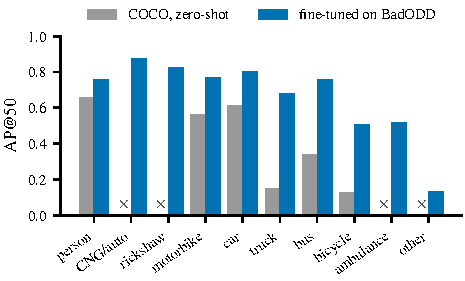
\includegraphics[width=\columnwidth]{per_class_ap}
\caption{Per-class AP@50 of RT-DETR-R18 on the official BadODD test split, COCO-pretrained (zero-shot) and
fine-tuned on the official training split. $\times$: a class the COCO model cannot output.}
\label{fig:perclass}
\end{figure}

\subsection{The leakage effect}
\label{sec:leak}
\TBD{[Pending: Kaggle runs \vid{rtdetr\_leaky}, \vid{rtdetr\_clean}, \vid{yolo\_leaky}, \vid{yolo\_clean}.]}
Table~\ref{tab:main} compares each detector trained on the leaky and the clean training set, on the same
1,019 test images. For RT-DETR, the leak raises mAP@50 by \TBD{D} (95\% CI \TBD{[a, b]}); the leaky model
scores higher in \TBD{k} of the 12 test videos. For YOLO11s the effect is \TBD{\ldots}.
\TBD{[Describe which classes gain most from the leak, using the per-class table from
\vid{compare\_runs.py}; and whether the effect is consistent across videos or driven by
\vid{maowa\_expressway2}.]}

\begin{table}[t]
\centering
\caption{Fine-tuned detectors. mAP@50 with 95\% CIs over test videos; $\Delta$ = leaky $-$ clean on the
same test images, with a paired CI.}
\label{tab:main}
\setlength{\tabcolsep}{4pt}
\begin{tabular}{@{}llcc@{}}
\toprule
Detector & Training set & Test set & mAP@50 \\
\midrule
\multirow{4}{*}{RT-DETR-R18} & official & official & 0.663 [0.607, 0.718] \\
 & leaky & paired & \TBD{x [a, b]} \\
 & clean & paired & \TBD{y [a, b]} \\
 & $\Delta$ & paired & \TBD{d [a, b]} \\
\midrule
\multirow{3}{*}{YOLO11s} & leaky & paired & \TBD{x [a, b]} \\
 & clean & paired & \TBD{y [a, b]} \\
 & $\Delta$ & paired & \TBD{d [a, b]} \\
\bottomrule
\end{tabular}
\end{table}

% =====================================================================
\section{Discussion and Limitations}

\textbf{What the official numbers mean.} A score on BadODD's official test split estimates how well a
detector finds objects in new frames of drives it has already seen, one sampling step from a training
frame. That is a valid question for some uses, but not the one a reader usually assumes: how the detector
does on a road it has not seen. \TBD{[Once Table~\ref{tab:main} is filled: state how much of the 0.663 the
paired experiment attributes to the leak.]}

\textbf{Recommendations.} For datasets built from video, split by video (or by location or day when videos
overlap), state the grouping, publish the split, and compute confidence intervals over the groups rather
than over images. For BadODD, our manifest provides such a split with the official proportions.

\textbf{Limitations.} We study one dataset and train each configuration once, so the intervals reflect test
sampling but not training randomness. The paired test set comes from 12 videos, and two of them supply 63\%
of its images. Its night share is lower than the official one (2.5\% against 16\%) because night footage
comes in a few long videos. BadODD's \emph{auto rickshaw} class covers gas and electric three-wheelers alike,
so we cannot report CNG auto-rickshaws and battery rickshaws separately. Finally, the leak we measure is the one
produced by BadODD's sampling rate; denser sampling would leak more, sparser less.

\textbf{Ethics.} BadODD is public under CC BY 4.0. This paper shows no dataset images; any that are added
must have faces and number plates blurred.

% =====================================================================
\section{Conclusion}
BadODD's official split places a near-copy of every test image in the training data. A video-held-out
re-split and a paired leaky/clean protocol make the effect measurable: \TBD{[one sentence with the RT-DETR
and YOLO11s effect sizes]}. We release the manifests and code so that future work on Bangladeshi road
detection can report scores that transfer to unseen roads.

\section*{Acknowledgment}
\TBD{[Funding and thanks, if any.]} \TBD{[AI disclosure required by IEEE, wording for the authors to confirm:
``Parts of the text and code were drafted with the assistance of Claude (Anthropic); the authors reviewed
and are responsible for all content.'']}

\bibliographystyle{IEEEtran}
\bibliography{refs}

\end{document}
